\documentclass[border=10pt]{standalone}
\usepackage[svgnames]{xcolor}
\usepackage{amsmath}
\usepackage{pgfplots}
\pgfplotsset{compat=newest}
\usepackage[sfdefault]{FiraSans}
\usepackage{FiraMono}
\renewcommand*\familydefault{\sfdefault}
\begin{document}
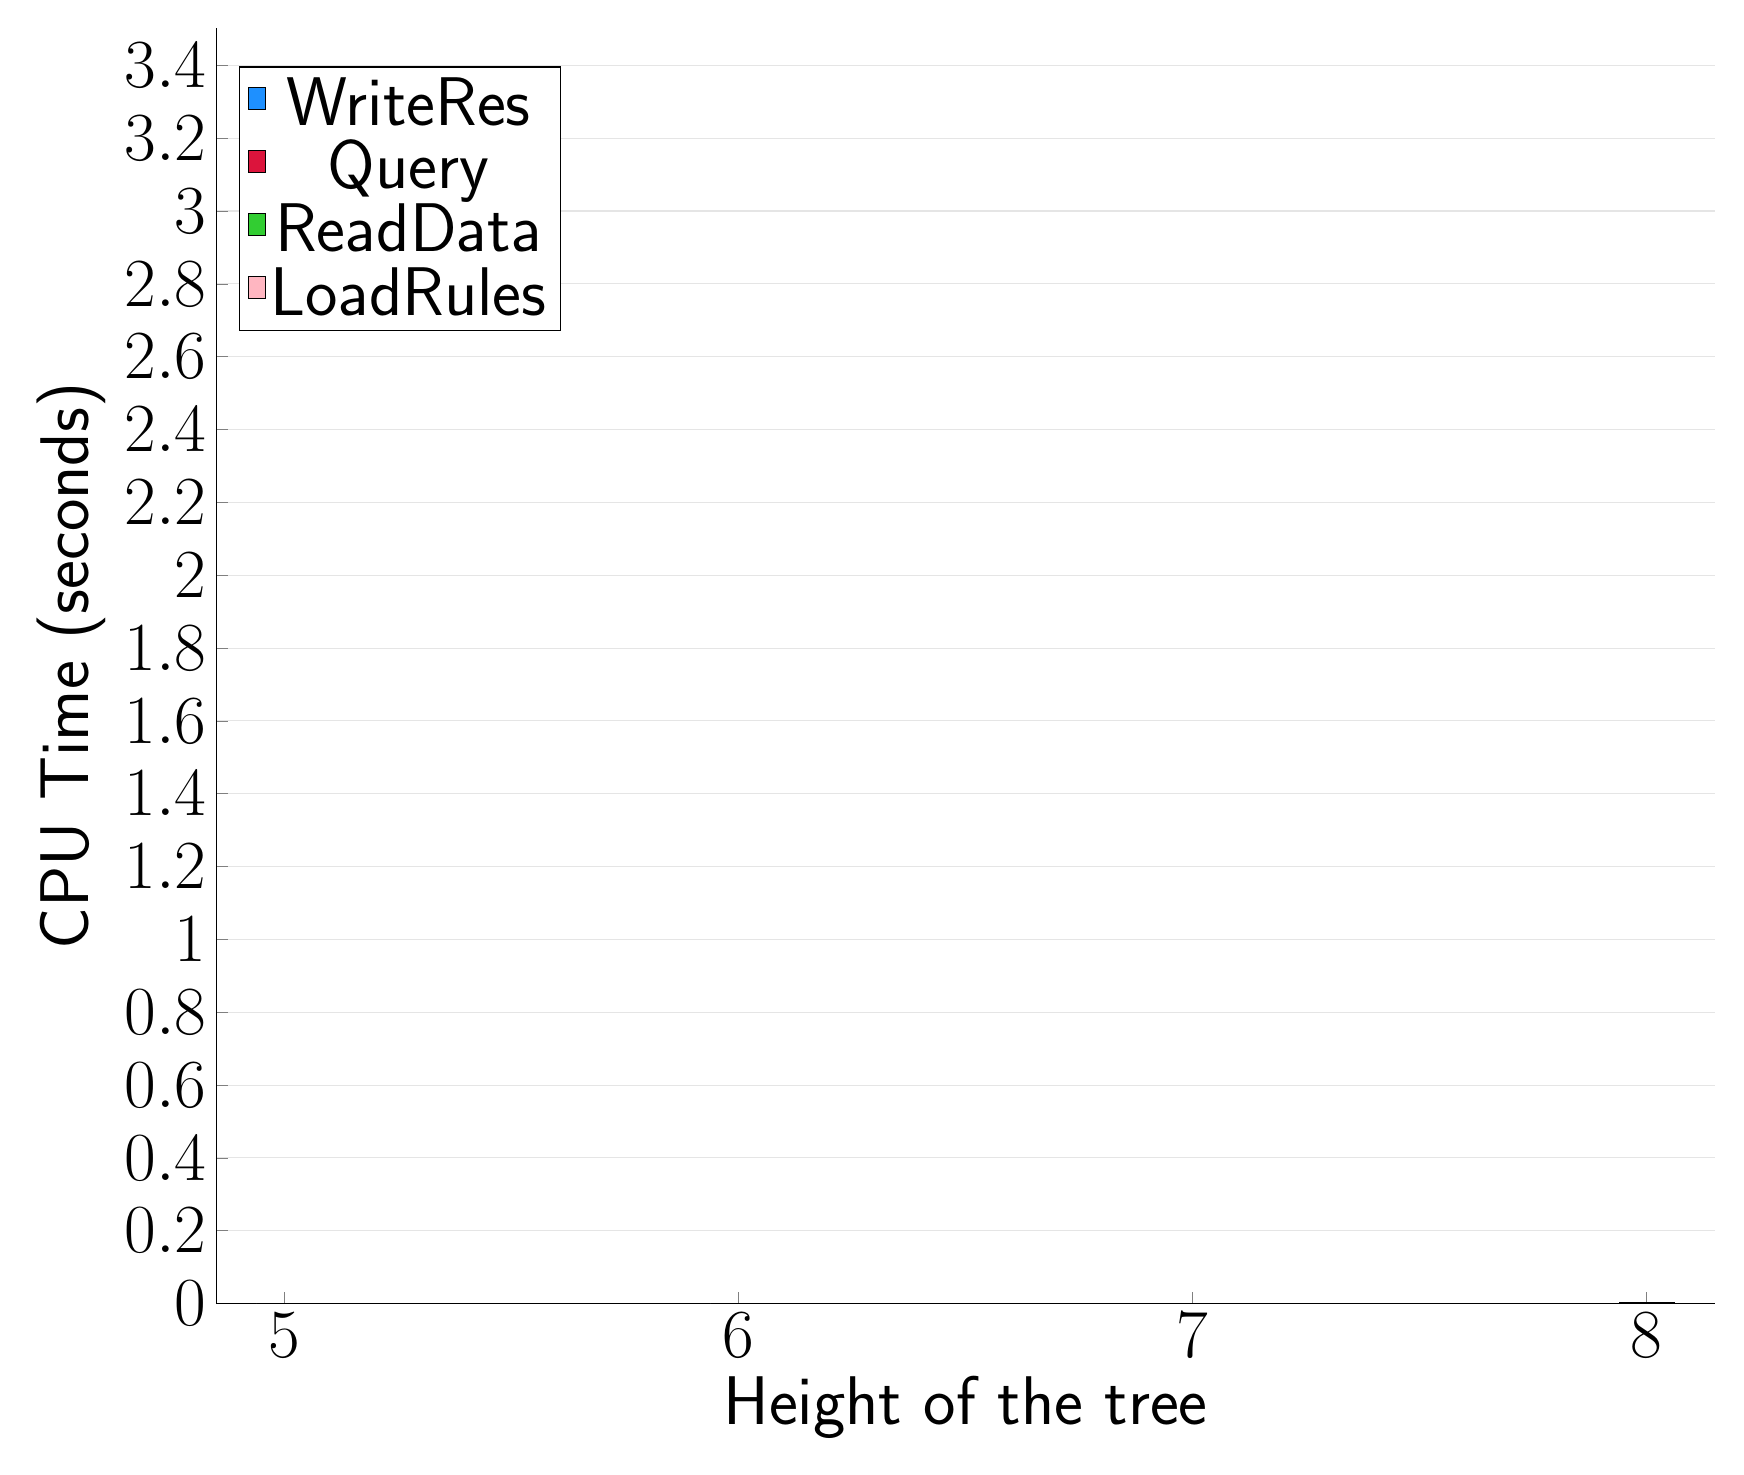
\begin{tikzpicture}
\begin{axis}[
   ybar stacked,
   width=1.7\textwidth,
   bar width=0.7cm,
   ymajorgrids, tick align=inside,
   major grid style={draw=gray!20},
   xtick=data,
   ymin=0, ymax=3.5020000000000002,
   axis x line*=bottom,
   axis y line*=left,
   enlarge x limits=0.05,
   legend style={
       at={(0.23, 0.97)},
       anchor=north east,
       legend columns=1,
       font=\Huge,
   },
   ylabel={CPU Time (seconds)},
   xlabel={Height of the tree},
   label style={font=\Huge},
   tick label style={font=\Huge},
]
\addlegendimage{fill=DodgerBlue, draw=black, line width=0.2pt}
\addlegendentry{WriteRes}
\addlegendimage{fill=Crimson, draw=black, line width=0.2pt}
\addlegendentry{Query}
\addlegendimage{fill=LimeGreen, draw=black, line width=0.2pt}
\addlegendentry{ReadData}
\addlegendimage{fill=LightPink, draw=black, line width=0.2pt}
\addlegendentry{LoadRules}
\addplot +[fill=LightPink, draw=black, line width=0.2pt] coordinates {
(5, 0.0006029000000000001)
(6, 0.0006119999999999998)
(7, 0.0006027999999999999)
(7, 0.0006178999999999999)
(7, 0.0006127000000000001)
(8, 0.0006044000000000004)
(8, 0.0006211000000000003)
(8, 0.0006079999999999998)
};
\addplot +[fill=LimeGreen, draw=black, line width=0.2pt] coordinates {
(5, 0.0001550999999999999)
(6, 0.00018570000000000018)
(7, 0.00024310000000000022)
(7, 0.00024140000000000007)
(7, 0.00024150000000000018)
(8, 0.0003522999999999995)
(8, 0.0003447999999999998)
(8, 0.0003491000000000001)
};
\addplot +[fill=Crimson, draw=black, line width=0.2pt] coordinates {
(5, 3.009999999999974e-05)
(6, 6.329999999999964e-05)
(7, 0.00015109999999999988)
(7, 0.00014750000000000022)
(7, 0.0001474999999999999)
(8, 0.0003725000000000001)
(8, 0.00036830000000000055)
(8, 0.0003709999999999997)
};
\addplot +[fill=DodgerBlue, draw=black, line width=0.2pt] coordinates {
(5, 0.00015820000000000027)
(6, 0.00030090000000000027)
(7, 0.0006467000000000006)
(7, 0.0006446999999999996)
(7, 0.0006536999999999999)
(8, 0.0014425)
(8, 0.0014566999999999996)
(8, 0.0014952000000000001)
};
\end{axis}
\end{tikzpicture}

\end{document}
